\documentclass[tikz,border=4pt]{standalone}
\usepackage{amsmath,amssymb}
\usetikzlibrary{positioning,fit,backgrounds,arrows.meta,decorations.pathreplacing}

\begin{document}
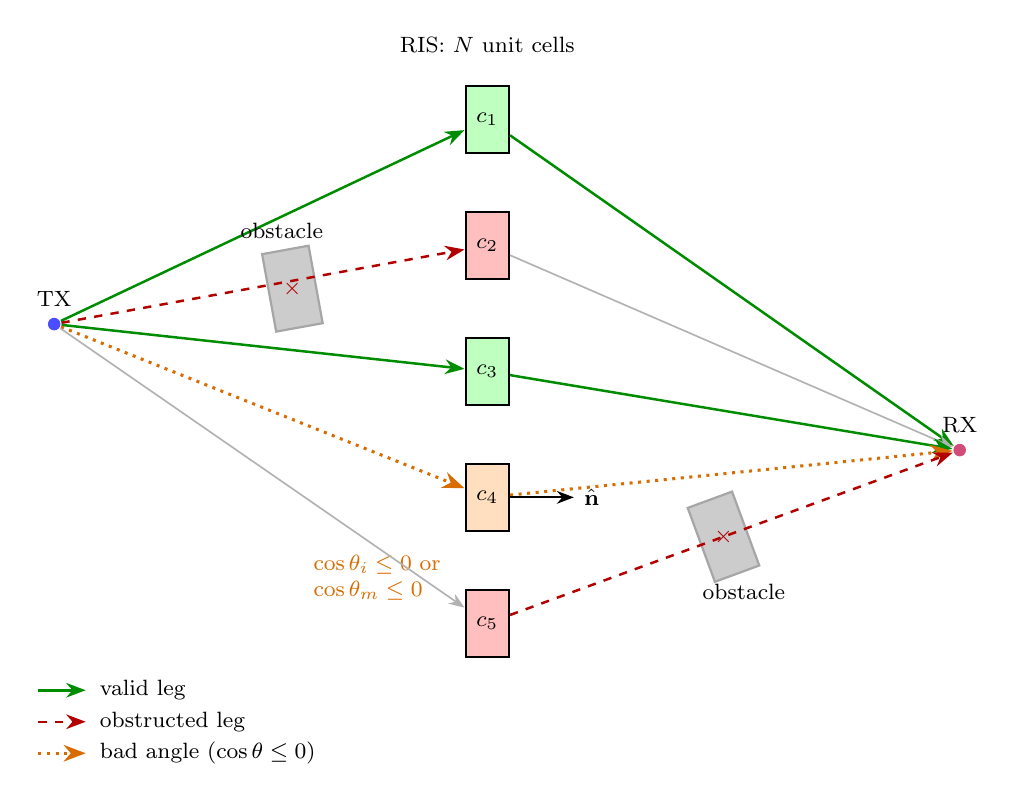
\begin{tikzpicture}[
  >=Stealth, thick, scale=1,
  validray/.style={-{Stealth}, green!55!black, line width=0.9pt},
  obstray/.style={-{Stealth}, red!70!black, dashed, line width=0.9pt},
  angray/.style={-{Stealth}, orange!85!black, dotted, line width=1.1pt},
  ghostray/.style={-{Stealth}, gray!60, line width=0.6pt},
  cellvalid/.style={fill=green!25, draw=black},
  cellobst/.style={fill=red!25, draw=black},
  cellang/.style={fill=orange!25, draw=black},
  every node/.style={font=\footnotesize}
]

  % TX and RX
  \node[circle, fill=blue!70, inner sep=1.6pt, label=above:{TX}] (tx) at (-5.5, 0.6) {};
  \node[circle, fill=purple!70, inner sep=1.6pt, label=above:{RX}] (rx) at (6.0, -1.0) {};

  % RIS surface: 5 cells stacked vertically at x=0, generously spaced
  \foreach \i/\y/\style in {1/3.2/cellvalid, 2/1.6/cellobst, 3/0.0/cellvalid, 4/-1.6/cellang, 5/-3.2/cellobst} {
    \node[\style, minimum width=0.55cm, minimum height=0.85cm] (c\i) at (0,\y) {$c_\i$};
  }
  \node[align=center] at (0,4.15) {RIS: $N$ unit cells};

  % --- Cell 1: fully valid path ---
  \draw[validray] (tx) -- (c1);
  \draw[validray] (c1) -- (rx);

  % --- Cell 2: obstructed TX->cell leg ---
  % Obstacle centered on, and rotated to, the TX--c2 ray so it visibly blocks it.
  \draw[fill=gray!40, draw=gray!70, rotate around={10.3:(-2.475,1.05)}]
        (-2.775,0.55) rectangle (-2.175,1.55);
  \node at (-2.61,1.79) {obstacle};
  \draw[obstray] (tx) -- (c2);
  \draw[ghostray] (c2) -- (rx);
  \node[red!70!black] at (-2.475,1.05) {$\times$};

  % --- Cell 3: fully valid path ---
  \draw[validray] (tx) -- (c3);
  \draw[validray] (c3) -- (rx);

  % --- Cell 4: bad incidence/reradiation angle ---
  \draw[angray] (tx) -- (c4);
  \draw[angray] (c4) -- (rx);
  \draw[->, black, line width=0.7pt] (c4) -- ++(1.1,0) node[right] {$\hat{\mathbf n}$};
  \node[orange!85!black, align=left, anchor=north] at (-1.4,-2.2) {$\cos\theta_i\le 0$ or\\$\cos\theta_m\le 0$};

  % --- Cell 5: obstructed cell->RX leg ---
  % Obstacle centered on, and rotated to, the c5--RX ray so it visibly blocks it.
  \draw[fill=gray!40, draw=gray!70, rotate around={20.2:(3.0,-2.1)}]
        (2.7,-2.6) rectangle (3.3,-1.6);
  \node at (3.26,-2.8) {obstacle};
  \draw[ghostray] (tx) -- (c5);
  \draw[obstray] (c5) -- (rx);
  \node[red!70!black] at (3.0,-2.1) {$\times$};

  % Legend
  \begin{scope}[shift={(-5.7,-4.6)}]
    \draw[validray] (0,0.55) -- (0.6,0.55); \node[anchor=west] at (0.65,0.55) {valid leg};
    \draw[obstray] (0,0.15) -- (0.6,0.15); \node[anchor=west] at (0.65,0.15) {obstructed leg};
    \draw[angray] (0,-0.25) -- (0.6,-0.25); \node[anchor=west] at (0.65,-0.25) {bad angle ($\cos\theta\le0$)};
  \end{scope}

\end{tikzpicture}
\end{document}
